% * * * * * * * * * * * * * * * * * * * * * * * * * * * * * * * * * * *
% *                             Thesis                                *
% *                 https://github.com/Jacopx/Thesis                  *
% * * * * * * * * * * * * * * * * * * * * * * * * * * * * * * * * * * *

\documentclass[%
    corpo=12pt,
    twoside,
%    stile=classica,
    oldstyle,
    autoretitolo,
    greek,
    evenboxes,
%    tipotesi,
]{toptesi}
%%%%%%%%%%%%%%%%%%%%%%%%%%%%%%%%%%%%%%%%%%%%%%%%%%%%

\usepackage[utf8]{inputenc}
\usepackage[T1]{fontenc}
\usepackage{lmodern}
\usepackage{hyperref}
\usepackage{graphicx}
\usepackage{subfigure}
\usepackage{booktabs}
\usepackage{amsfonts}
\usepackage{amsmath}
\usepackage{amssymb}
\usepackage{bm}
\usepackage{listings}

\hypersetup{%
    pdfpagemode={UseOutlines},
    bookmarksopen,
    pdfstartview={FitH},
    colorlinks,
    linkcolor={blue},
    citecolor={blue},
    urlcolor={blue}
  }

%%%%%%% Definizioni locali

\interlinea{1.5} 


\begin{document}

\ateneo{Politecnico di Torino}
%
% Non tutte le università hanno un nome proprio
%\nomeateneo{Sede di Torre Elettra}
%
% \FacoltaDi{Faculty of Computer Engineering}% lo spazio finale correttamente sparisce

\titolo{Predizione di difettosità nello sviluppo software attraverso machine learning}
\sottotitolo{Artificial Intelligence applied to Software Engineering}

%
%%%%%%% Corso degli studi
\corsodilaurea{Ingegneria Informatica}% per la laurea
%\corsodidottorato{Meccanica}% per il dottorato

\renewcommand*\IDlabel{}
%
\candidato{Jacopo \textsc{Nasi} [255320]}

%%%%%%% Relatori o supervisori
\relatore{prof.~Maurizio \textsc{Morisio}}

%%%%%%% Tutore
\tutoreaziendale{dott.\ Davide \textsc{Piagneri}}

\sedutadilaurea{\textsc{Aprile} 2020}


%%%%%%% Logo della sede
\logosede{polito}

%%%%%%% OFFSET
%\setbindingcorrection{3mm}

%\english

\iflanguage{english}{%
	\retrofrontespizio{This work is subject to the Creative Commons Licence}
	\DottoratoIn{PhD Course in\space}
	\CorsoDiLaureaIn{Master degree course in\space}
	\NomeMonografia{Bachelor Degree Final Work}
	\TesiDiLaurea{Master Degree Thesis}
	\NomeDissertazione{PhD Dissertation}
	\InName{in}
	\CandidateName{Candidates}% or Candidate
	\AdvisorName{Supervisors}% or Supervisor
	\TutorName{Tutor}
	\NomeTutoreAziendale{Internship Tutor}
	\CycleName{cycle}
	\NomePrimoTomo{First volume}
	\NomeSecondoTomo{Second Volume}
	\NomeTerzoTomo{Third Volume}
	\NomeQuartoTomo{Fourth Volume}
	\logosede{polito}% or comma separated list of logos
}{}
%%%%%%%%%%%%%%%%%%%%%%%%%%%%%%%%%%%%%%%%%

\frontespizio
\summary
Ogni giorno migliaia di commit vengono eseguiti, ognugno di loro contiene molte informazioni: file modificati, modifiche, commenti, registri di test e molto altro. Una strutturata e corretta gestione delle piattaforme di concontrollo sorgente permette l'estrazione di dati utili analizzabili utilizzando modelli statistici di intelligenza artificiale.\\
Al fine di poter correttamente utilizzare questi dati sono necessari alcuni step preliminari: la prima fase riguarda l'analisi della struttura dati al fine di permettere l'estrazione di tutte le possibili informazioni, successivamente la pre-elaborazione per rimuovere informazioni di inutili e di disturbo, con i dati puliti è possibile procedere con l'estrazione di dati combinati, come la seniority degli sviluppatori, una lista di parole dei componenti modificati, la versione ed altre informazioni di carattere più matematico. L'ultima fase prevede la sostituzione dell'etichetta testuale relativa alla priorità con un valore numerico corrispondende al valor medio della distribuzione della durata di quella etichetta, questo valore prenderà il nome di severity. I dati verranno poi aggregati per settimana.
Una volta generati i dati verranno utilizzati per allenare tre differenti modelli: Random Forest, Gradient Boosting e Reti Neurali. L'allenamento sarà gestito in tre differenti modalità: la prima allena e predice utilizzando lo stesso filone di dati, la seconda, cross-version, prevede che il modello venga allenato su dati relativi ad alcune versione del progetto per poi effettuare la predizione sulle successive, la terza, cross-project, allena il modello con dati relativi ad un progetto per poi prevedere l'andamento di uno differente.\\
Tutti le tipologie ottengono dei buoni risultati, il migliore è quello cross-project che riesce ad ottenere una precisione maggiore del 90\% fino a quattro settimane e comunque maggiore del 70\% fino a 20 settimane.


\acknowledgements

Un ringraziamento speciale a Smirnuff ed i suoi cavalieri, luce della mia battaglia.

\indici

\mainmatter

% #######################################
% #            Introduction             #
% #######################################

\chapter{Introduzione}
\label{chap:intro}
\section{Problema Generale}
Lo sviluppo software non si presenta molto differente dallo sviluppo di qualsiasi altro prodotto, dopo una fase iniziale di progettazione lo sviluppo del codice può avere inizio, durante esso emergeranno sistematicamente dei problemi che dovranno essere risolti prima della consegna della versione finale.\\
Ogni progetto software è costituito da diversi commit per giorno, ognugno di essi contiene innumerevoli informazioni le quali possono essere utilizzate per analisi statistiche. La predizione della difettosità può migliorare enormemente il processo di sviluppo, allocando un corretto numero di sviluppatori per risolvere le problematiche e riducendo quindi le tempistiche per la correzione. Anche il machine learning può essere utilizzato per la predizione dei difetti.\\
La predizione è uno strumento sempre più utilizzato a livello industriale, un corretto utilizzo può generare enormi benifici a livello produttivo, permettendo la riduzione di sprechi, l'ottimizzazione delle vendite e tante altri vantaggi. Lo sviluppo di progetti di natura informatica è sempre di più centrale all'interno della nostra società attuale, anche questo processo potrebbe trarre beneficio dai vantaggi della predizione. L'implementazione di tecniche statistiche viene in supporto, vista la natura intellettuale della programmazione, nello generazione di predizioni utili.

\section{Strumenti utilizzati}
Lo sviluppo di questo progetto a richiesto l'utilizzo di diversi strumenti, di seguito una lista degli stessi:

\paragraph{\href{https://www.python.org/}{Python}} Il linguaggio di programmazione principale, utilizzato per la gestione dei dati, l'estrazione di informazioni, l'applicazione di algoritmi matematici e l'interazione con altri software. Nello specificio la versione utilizzata è stata la v3.7.0

\paragraph{\href{https://pandas.pydata.org/}{Pandas}} Libreria open source ad alte prestazioni, con semplici strutture e strumenti adatti all'analisi dati attraverso Python.

\paragraph{\href{https://numpy.org/}{NumPy}} Libreria per il calcolo scientifico attraverso Python.

\paragraph{\href{https://matplotlib.org/}{Matplotlib}} Libreria per il disegno di grafici 2D in Python.

\paragraph{\href{https://seaborn.pydata.org/}{Seaborn}} Libreria avanzata per il disegno 2D in Python.

\paragraph{\href{https://www.tensorflow.org/}{Tensorflow}} Piattaforma per machine learning.

\paragraph{\href{https://keras.io/}{Keras}} API di alto livello per reti neurali.

\paragraph{\href{https://scikit-learn.org/stable/}{SciKit-Learn}} Strumenti e librerie per machine learning.

\paragraph{\href{https://gitlab.com}{GitLab}} Piattaforma di sourcing basata su Git. Utilizzata per il codice sorgente del progetto.
% \url{https://gitlab.com/EiS-Projects/analytics/temp/thesisProjectJN}.

\paragraph{\href{https://github.com}{GitHub}} Piattaforma di sourcing basata su Git. Utilizzata per il calendario e elaborato testuale:
\begin{itemize}
  \item Tesi: \url{https://github.com/Jacopx/Thesis}
  \item Calendario: \url{https://github.com/Jacopx/ThesisCalendar}
\end{itemize}

\paragraph{\href{https://www.jetbrains.com/}{JetBrains IDEs}} IDE per lo sviluppo di diversi linguaggi di programmazione, gratuita per gli studenti:
\begin{itemize}
  \item PyCharm: \url{https://www.jetbrains.com/pycharm/}
  \item DataGrip: \url{https://www.jetbrains.com/datagrip/}
\end{itemize}

% #######################################
% #            State of art             #
% #######################################
\chapter{Stato dell'arte}
\section{Lavori correlati}
Parlando di altri lavori su simili tematiche.

% #######################################
% #              Datasets               #
% #######################################

\chapter{Dati}
\label{chap:dataset}
Le seguenti sezioni analizzeranno le basi di dati utilizzate in questo progetto.
\section{SEOSS33}
SEOSS33\cite{SEOSS33} è una \href{https://doi.org/10.7910/DVN/PDDZ4Q}{base dati} collezionante errori, issue e tante altre informazioni a proposito di 33 progetti open source. I dati sono stati tutti collezionati estraendo le informazioni dalle piattaforme di controllo del codice sorgente, Version Control System (VCS), come GitHub e dalle piattaforme per la gestione dello sviluppo, Issue Tracking System (ITS), come Jira di Atlassian.\\
Ad oggi nessun altro progetto di ricerca, su questi dati, è stato effettuato.\\
Ogni progetto prevede una propria linea durante la fase di sviluppo, tutte le metodologie e linee guida sono alla base degli studi di ingegneria del software. Tuttavia è possibile unificare ed accorpare secondo una categorizzazione standar molte delle differenze specifiche. Lo svilluppo della base dati SEOSS33 mira proprio alla creazione di un serie di dati generalizzati e fruibili attraverso medesime procedure senza la necessità di adattarsi alle specifiche caratteristiche di ogni singolo progetto.\\
Il mondo open source presenta una quantità pressochè infinita di differenti software, parte del progetto in questione è stata dedicata alla selezione dei software da analizzare per l'inserimento nella base dati condivisa, per questo motivo sono state definite alcune carattestiche che accomunassero i vari progetti in modo da costituire una base: discretamente omogenea a livello di dimensionalità, ma con differenze struttuali utili per successive analisi come quella relativa a questo progetto. Il requisito principiale riguardava il linguaggio di programmazione, considerare progetti sviluppati per la maggior parte in un singolo linguaggio di programmazione permette di ridurre la variabilità interna ad ogni singolo progetto. Vista la natura di analisi attraverso il machine learning, un'altra importante carattestica riguardava il numero di issue, il quale doveva essere sufficientemente elevato. I progetti, oltre a dover essere attualmente in sviluppo, dovevano presentare un età di almeno 3 anni. La definizione di tutti questi parametri a permesso di generare una base dati contenente 33 progetti simili come struttura ma con caratteristiche differenti.\\
Lo sviluppo del presente progetto di tesi si è concentrato solamente su cinque di questi schemi, sono stati scelti i progetti più grossi e quelli in sviluppo dal maggior tempo, nello specificio i selezionati sono riportati in tabella \ref{tab:seoss33_selected}:
\begin{center}
  \captionof{table}{Project data distribution} \label{tab:seoss33_selected}
  \begin{tabular}{ |c|c|c| }
     \hline
     \textbf{Project} & \textbf{Month} & \textbf{Issue} \\
     \hline
     \hline
     Hadoop & 150 & $39086$ \\
     Hbase & 131 & $19247$ \\
     Maven & 183 & $18025$ \\
     Cassandra & 106 & $13965$ \\
     Hive & 113 & $18025$ \\
     \hline
  \end{tabular}
\end{center}

Al fine di generalizzare le specifiche differenze, le varie issue: \textit{New Feature}, \textit{Bug Report}, ecc... Sono state mappate su cinque categorie:
\begin{itemize}
  \item Bug: Un problema che previene il funzionamento del prodotto
  \item Feature: Una nuova funzionalità del prodotto
  \item Improvement: Un miglioramento di una funzionalità già esistente
  \item Task: Un compito necessario
  \item Other: Vario
\end{itemize}

La figure \ref{fig:prior} visualizza la distribuzione, rispetto le varie categorie, del numero di issue per ogni progetto.

\begin{figure}[!ht]
  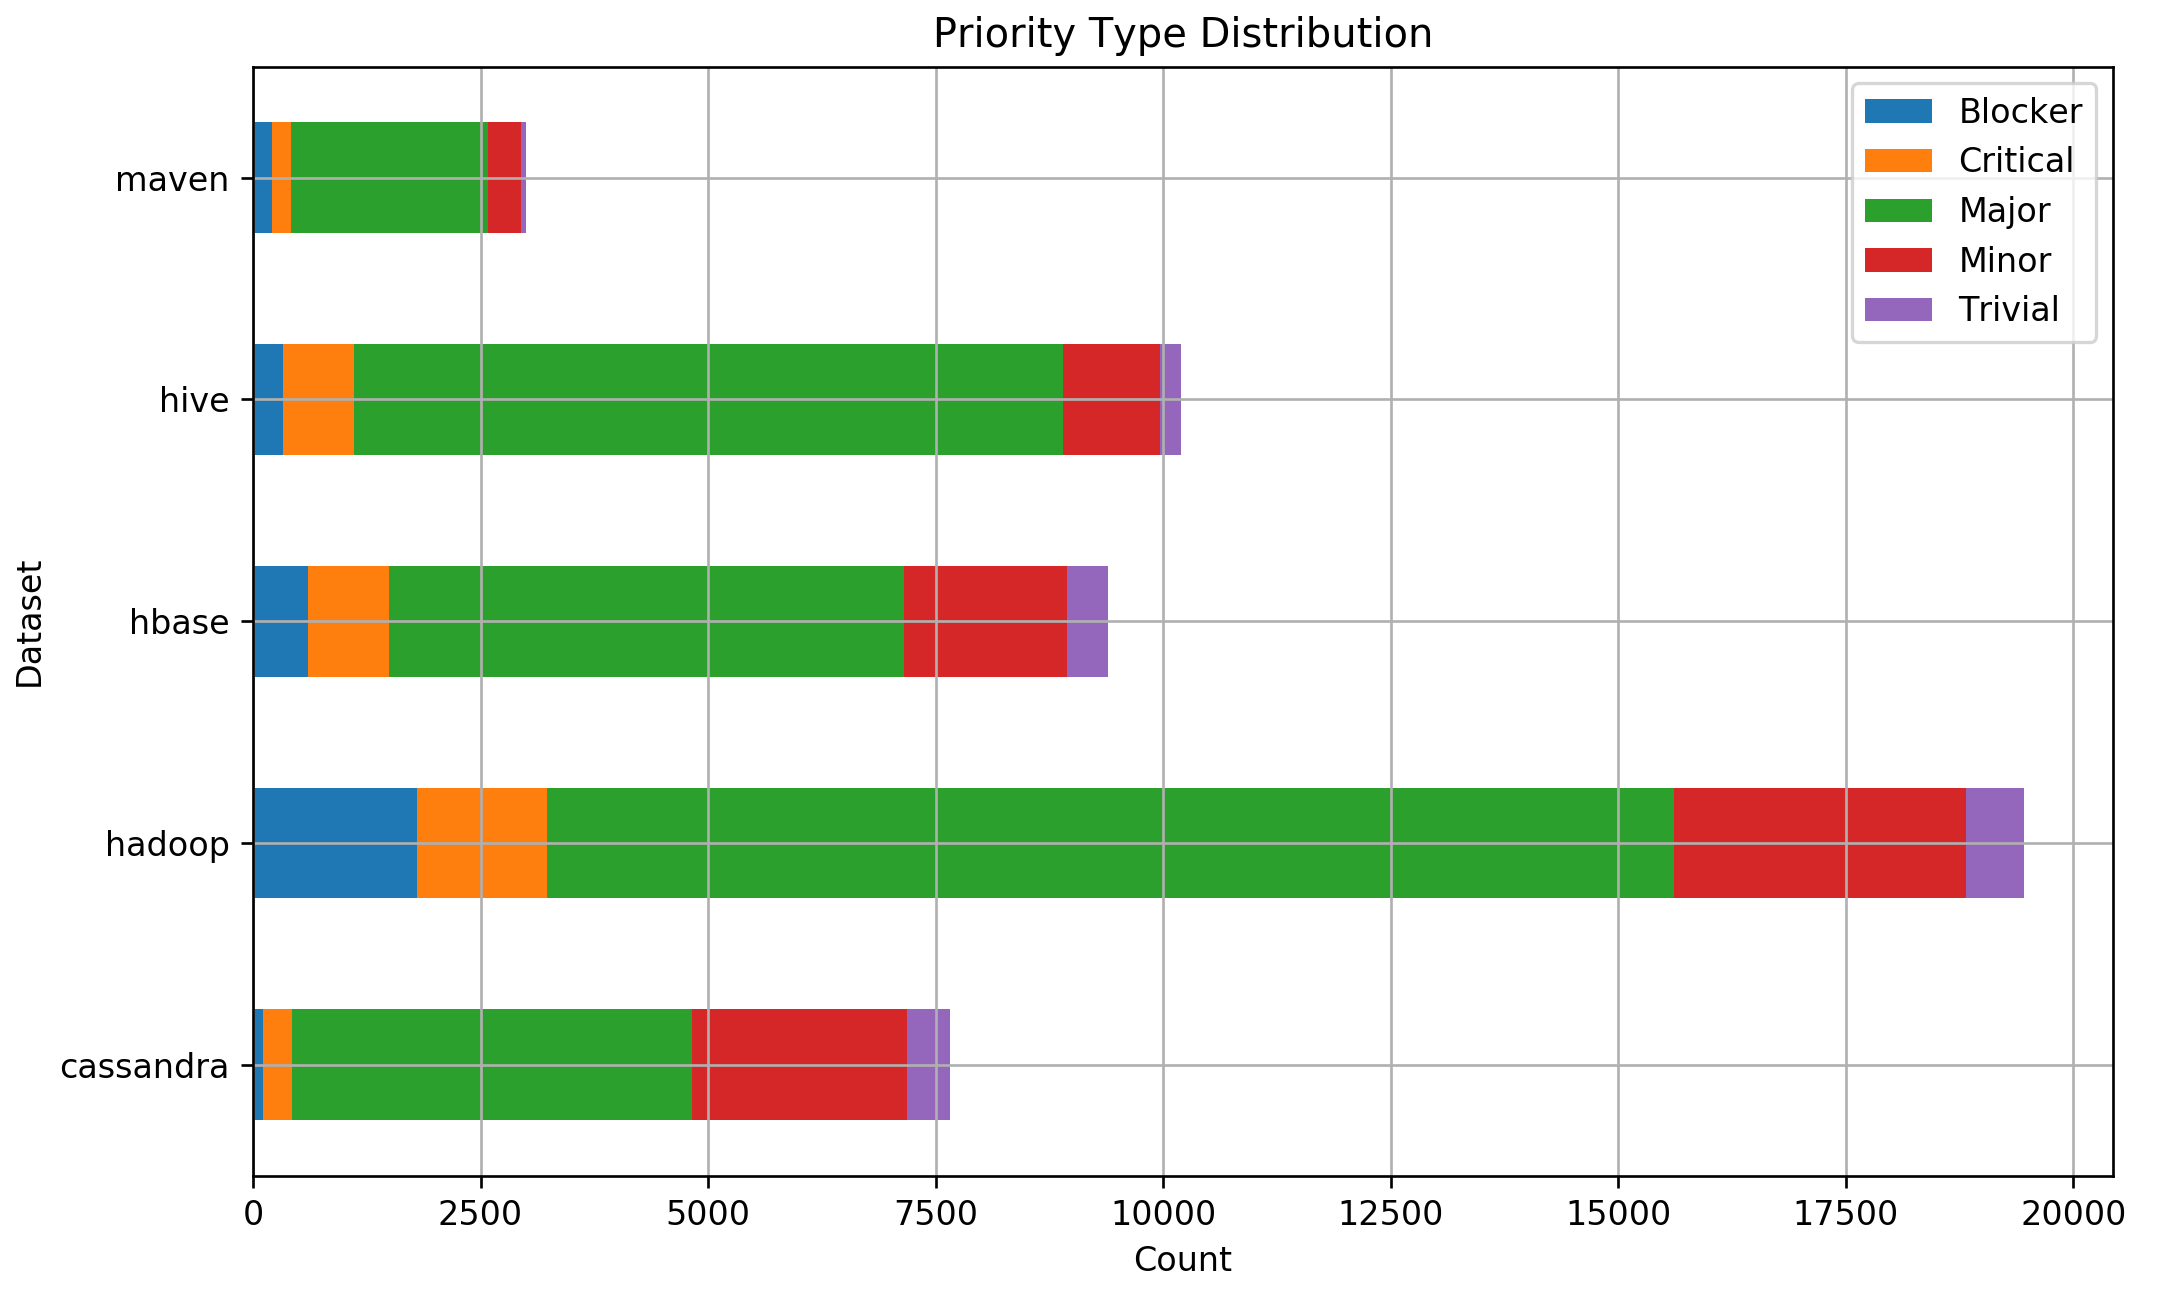
\includegraphics[width=\linewidth]{figure/prior.png}
  \caption{Distribuzione issue per progetto}
  \label{fig:prior}
\end{figure}

Per poter estrarre ed utilizzare al meglio i dati è necessario conoscere al meglio la struttura contenitore.
I dati relativi ad ogni software sono salvati in un file SQLITE, un database SQL offline che permette l'accesso sfruttando le potenzialità delle query, senza la necessità di un server vero e proprio. La figura \ref{fig:seoss33_db} riporta lo schema integrale della struttura.\\
Tutto il modello si basa sulla sua entità centrale, la issue, ovvero l'attività di segnalazione che è stata creata da uno sviluppatore per gestire una problematica. Ognugna di queste issue è caratterizzata dal proprio \textit{issue\_id} il quale ne rappresenta la chiave primaria ed univoca, normalmente è strutturata con il nome del progetto seguito da un numero progressivo. La tabella relativa alle issue contiene ulteriori informazioni direttamente correlate, la tipologia, la priorità, le informazioni temporali di apertura, aggiornamento e chiusura della stessa, un breve riassunto della problematica, lo stato e le informazioni relative allo sviluppatore che l'ha aperta. Direttamentamente collegate, tramite la chiave primaria, vi sono le tabelle contenenti i commenti \textit{issue\_comment}, la versione \textit{issue\_fix\_version}, il componente modificato \textit{issue\_component} ed la tabella \textit{change\_set\_link} la quale collega i vari commit alle issue. Durante l'estrazione delle varie informazioni sono state utilizzate tute le tabelle ad esclusione di \textit{issue\_link} la quale viene utilizzare per correlare le differenti issue tra di loro.

\begin{figure}[!ht]
  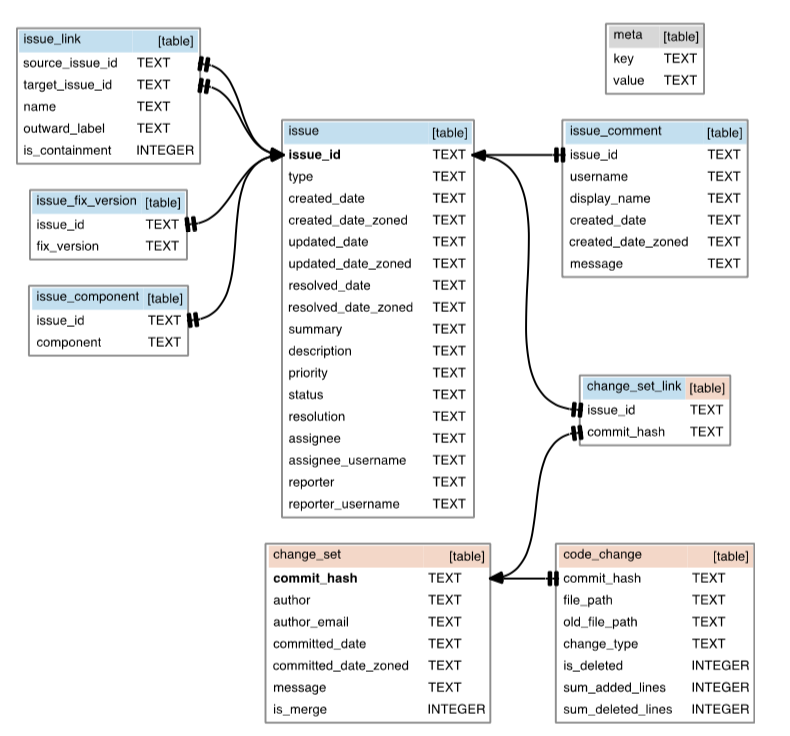
\includegraphics[width=\linewidth]{figure/seoss33_db_schema.png}
  \caption{SEOSS33 data model}
  \label{fig:seoss33_db}
\end{figure}


% #######################################
% #          Machine Learning           #
% #######################################

\chapter{Machine Learning}
\label{chap:ml}
\section{Introduzione}
Machine learning (ML) is the scientific study of algorithms and statistical models that computer systems use to perform a specific task without using explicit instructions, relying on patterns and inference instead. The word ML is almost in the public domain now, in the last decades the usage of this kind of algorithm has dramatically risen although most of it had already been developed for years. The main reason is the increase in the computational capacity of the systems.\\
There are two types of systems:
\begin{itemize}
  \item Knowledge-based: Acquisition and modeling of common-sense knowledge and expert knowledge (from rules to facts)
  \item Learning: Extraction of knowledge and rules from example/experience (from facts to rules)
\end{itemize}
All the machine learning techniques try to develop systems similar to the second definition. ML algorithms can be divided into three categories: supervised, unsupervised and reinforcement learning. The first will be used to predict class based on previous knowledge, the second tries to labeling data without a priori experience and the third bases it is learning on action reward.\\
There a lot of different models available, the following chapters will focus on the models used in this project.

\paragraph{Supervised Learning}
is a powerful technique to process labeled, which is a dataset with that has been classified, to infer a learning algorithm. This dataset is used as a basis to predict and learn how to predict unlabeled data. There are two types of supervised learning, classification, and linear regression. The goal of classification models is to predict categorical class labels of new instances, based on a training set of past observations. The classification can be binary or multi-class. Instead, regression, aim to predict continuous outcome, it tries to find mathematical relationships between variables to predict the target with a reasonable level of approximation. Our project is only focused on regression, classification will not be further discussed.

\section{Ensable Methods}
All the supervised learning method used are based on ensable, the basic idea is to merge multiple, different, hypothesis to improve the quality of the prediction, for example, the random forest or gradient boosting are ensable of multiple decision trees. The following paragraphs will deal with the models used specifically.

\paragraph{Random Forest}
Random Forest (RF) is a supervised learning algorithm that makes use of ensable learning method for classification and regression. They are built by combining the predictions of several trees, each of which is trained independently and the prediction of the trees are combined through averaging \cite{RF_theory}. A visualization of an RF is shown in figure \ref{fig:rf}.

\begin{figure}[!ht]
  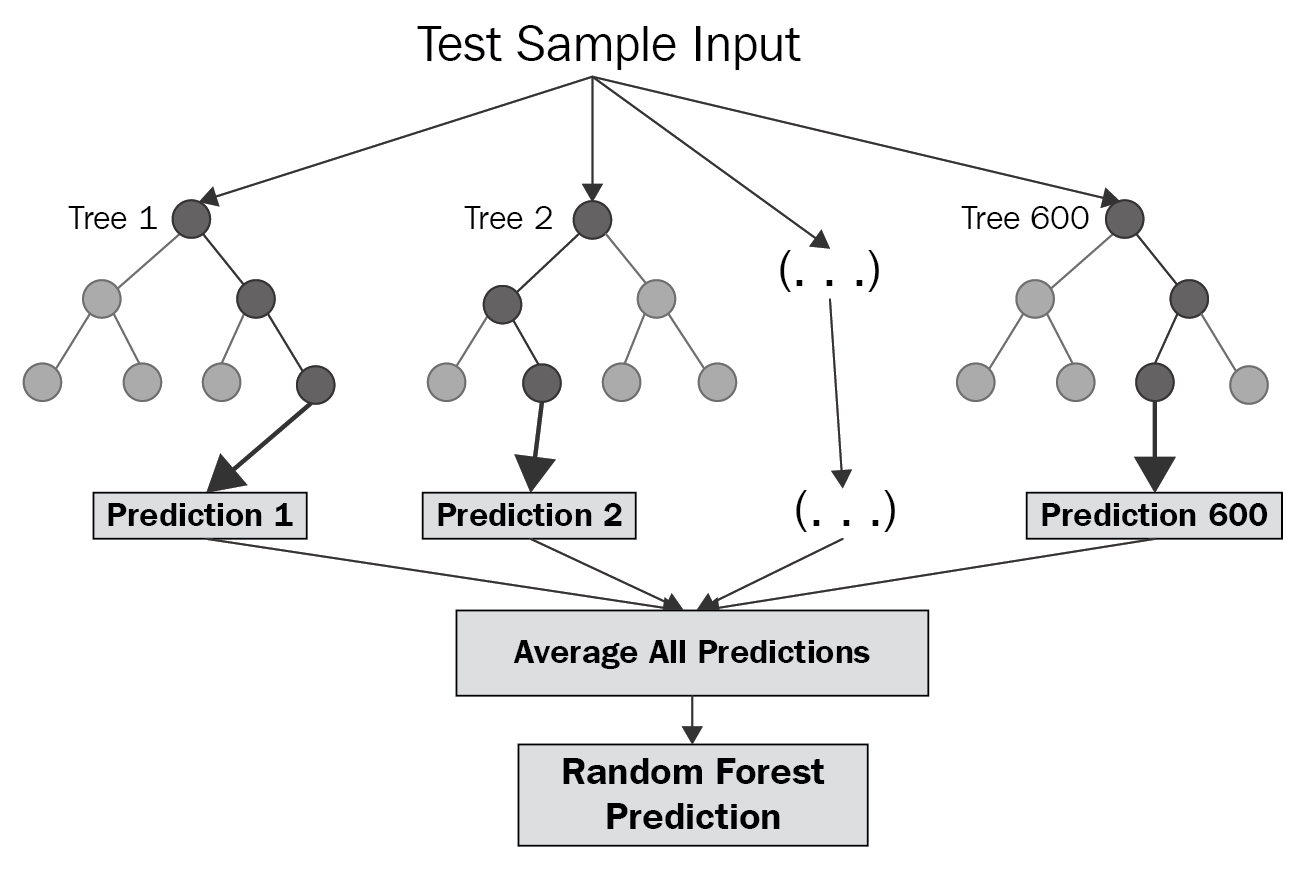
\includegraphics[width=\linewidth]{figure/rf.png}
  \caption{Random Forest simplified scheme \cite{rf}}
  \label{fig:rf}
\end{figure}

Three parameters are important to define the RF: (1) the methods for splitting the leaves, (2) the type of predictor to use in each leaf, and (3) the method for injecting randomness.
Splitting of requires the selection of shape and a method for evaluating the quality of each candidate. Typical choices are axis-aligned splits, where data is routed to sub-tree depending on a threshold. The threshold can be chosen randomly by a leaf optimization function. After the generation of different candidate splits a choosing criterion must be defined in order to split the leaf. One of the simplest strategies is to choose among the candidates uniformly at random, otherwise, it is possible to select the candidate split which optimizes a purity function (information gain for example) over the leaf that would be created.
The most common predictors, for each leaf, are the average response over training points that fall in that leaf.
The injection of randomness can happen in different ways, the size of candidate splits, coefficients for random combinations, etc\dots In any case, the thresholds can be also defined randomly or by optimization over data. Another solution is to build a tree using bootstrapped or sub-sampled dataset.\\
The training phase is performed independently by each tree by exploiting an assignment in structure and estimation points to respectively change the shape of the tree and to improve the estimator fit.\\
Once the forest has been trained it can be used to make predictions for unlabeled data points. In the prediction phase, every single tree, independently make its own prediction than an average of all the trees is computed to make a single outcome value. The contribution of each tree to the final value is the same.\\
Out implementation uses Random Forest developed by SciKit-Learn v0.21:
\begin{lstlisting}[language=python, frame=single]
  from sklearn.ensemble import RandomForestRegressor
\end{lstlisting}
The specific parameters of the model will be explained during the \autoref{chap:forecasting} about forecasting.
% To make predictions for a query point $x$, each tree independently predicts
% \begin{center}
%   \begin{equation}
%     f^{j}_{n}(x) = \frac{1}{N^{e}(A_{n}(x))} \sum_{I_{i}=e}^{Yi \in A_{n}(x)} Y_{i}
%   \end{equation}
% \end{center}
% and the forest averages the prediction of each tree
% \begin{center}
%   \begin{equation}
%     f^{(M)}_{n}(x) = \frac{1}{M} \sum_{j=1}^{M} f^{j}_{n}(x)
%   \end{equation}
% \end{center}

\paragraph{Gradient Boosting Machines}
Gradient Boosting Machines (GBM) are a family of powerful machine learning techniques that have shown considerable success in a wide range of practical applications. They are highly customizable to the particular needs of the application, line being learned with respect to different loss functions \cite{gbm}. Techniques like RF rely on simple averaging of model in the ensable. The family of boosting methods is based on a different constructive strategy of ensemble formation. Boosting add, sequentially, new models to the ensable. In GBM the learning phase consecutively fits new models to improve the accuracy of the estimations. Ideally, they construct new basic layers,  decision trees of fixed size, to be maximally correlated with the negative gradient of the loss function of the ensable. The loss function should be chosen by the developer, even ad-hoc loss function could be implemented. The attempt is to solve this minimization problem numerically via steepest descent \cite{ensable}.\\
This high flexibility of GBM makes them really customizable to any kind of task. Given its simplicity, a lot of experimentation can be performed over the model.\\
Our project implement Gradient Boosting Decision Tree (GBDT) developed by SciKit-Learn v0.21:
\begin{lstlisting}[language=Python, frame=single]
  from sklearn.ensemble import GradientBoostingRegressor
\end{lstlisting}

\section{Reti Neurali}
A Neural Network (NN) is a machine learning approach inspired by the way in which the brain performs a particular learning task, network of simple computational units (neurons) connected by links (synapses). The knowledge about the learning task is given in the form of training examples, the inter neurons connection strengths (weights) are used to store the acquired information. During the learning process, the weights are modified in order to model the particular learning task correctly on the examples.\\
The learning phase can be both supervised or unsupervised. Supervised is used for pattern recognition, regression and similar is trained using data with both input and desired output. Unsupervised instead is mainly used for clustering and the learning is made using unlabeled training examples. Only supervised one will be evaluated.\\
There are three main classes of network architectures:
\begin{itemize}
  \item Single-layer feed-forward
  \item Multi-layer feed-forward
  \item Recurrent
\end{itemize}
A standard architecture is composed of three different layers, \textit{input units}, \textit{hidden units} and \textit{output units}, all the layers are linked with the learning algorithms used to train. An example of a complete multi-layer network in \ref{fig:mlff}.

\begin{figure}[!ht]
  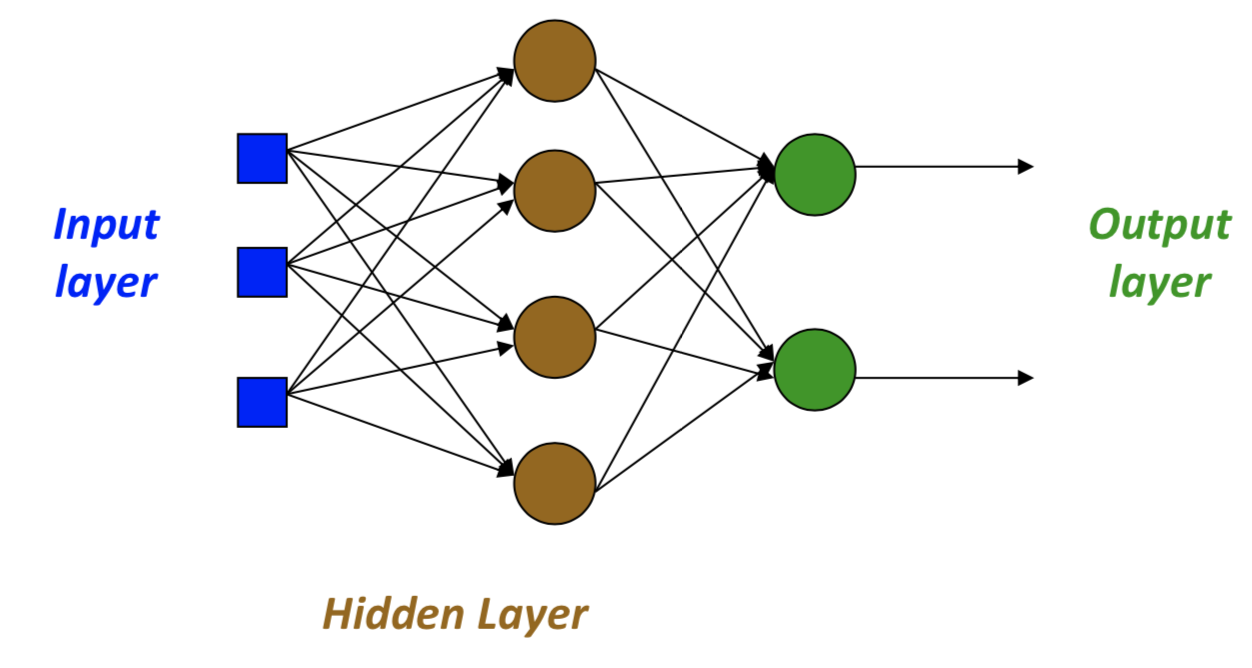
\includegraphics[width=\linewidth]{figure/feed_foward.png}
  \caption{Multi-layer feed-forward NN}
  \label{fig:mlff}
\end{figure}

The neuron is the basic processing unit of the network, which received the inputs. Each input is combined with its internal state and an optional activation function, it produces an output value that will be passed to the next layers. The weights, defined during the training phase, corresponding to the importance of the connection. The different inputs are summed using a weighted sum:
\begin{center}
  \begin{equation}
    u = \sum^{m}_{j=1} w_{j}x_{j}
  \end{equation}
\end{center}
The computed value is than scaled using an activation function $\varphi$ for limiting the amplitude of the output of the neuron by applying the function:
\begin{center}
  \begin{equation}
    y = \varphi(u + b)
  \end{equation}
\end{center}
Where $b$ represent the bias, an external parameter of the neuron, $y$ represent than the output value for the next level. An example of the structure can be found in figure \ref{fig:neuron}.

\begin{figure}[!ht]
  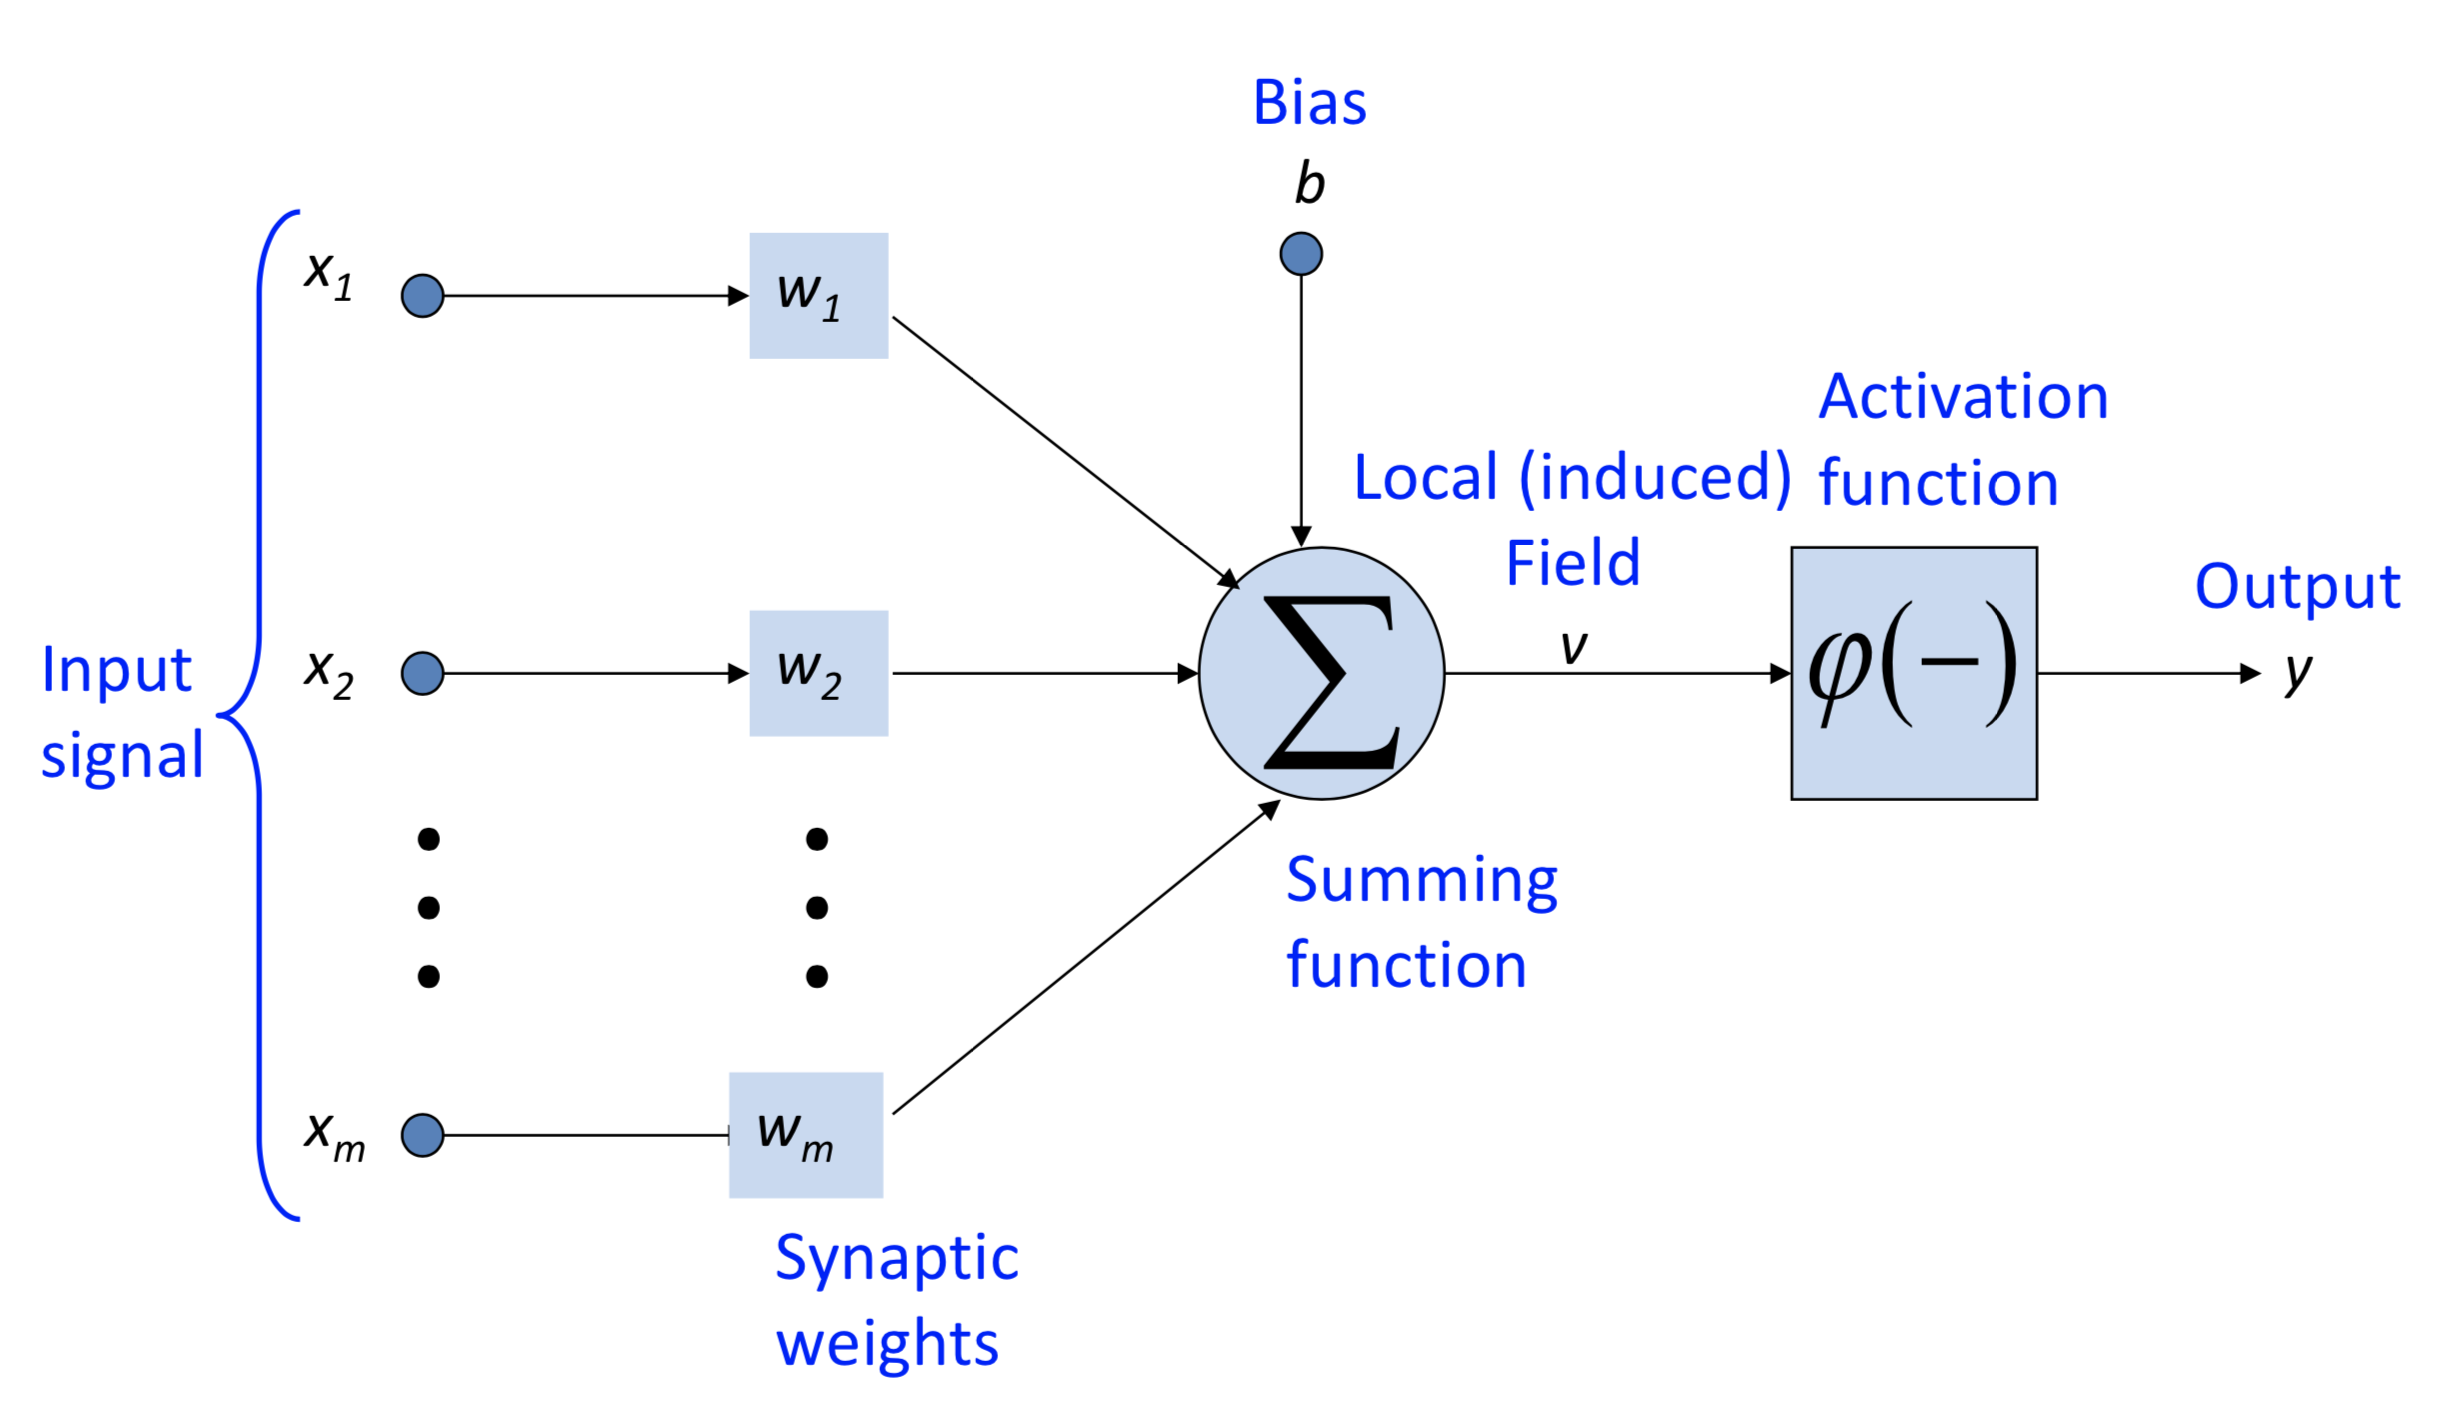
\includegraphics[width=\linewidth]{figure/neuron.png}
  \caption{Neuron view}
  \label{fig:neuron}
\end{figure}

Several different functions can be used to activate the neurons, they are trying to emulate the typical response of a biological neuron and its different activation methods. The most common are: linear, step, relu and sigmoid.
Each function behaves differently with different peculiarities and critical issues, there are two main types, linear and non-linear.

\paragraph{Step} is a binary, linear and threshold-based activation function, figure \ref{fig:step}. When the input is above or below a defined threshold, the neuron is activated and pass the same input value to the next layer. The main drawback is that not allow multiple-value output.

\paragraph{Linear} is of course a linear activation function that take the form:
\begin{center}
  \begin{equation}
    f(x) = x
  \end{equation}
\end{center}
This function takes the input and, by multiplying it by the weight of the neuron, it calculate the output. Respect the step function allows multiple-value output, but there are two major problems: it is not possible to use backpropagation (treated later) to train the network because the derivative function is constant and is not related to the input. The other problem is that linear function collapses all the layers into once because the last layer will be a linear combination of the first in any case. Figure \ref{fig:linear} show the curve.

\begin{figure}
  \centering
  \begin{minipage}{.5\textwidth}
    \centering
    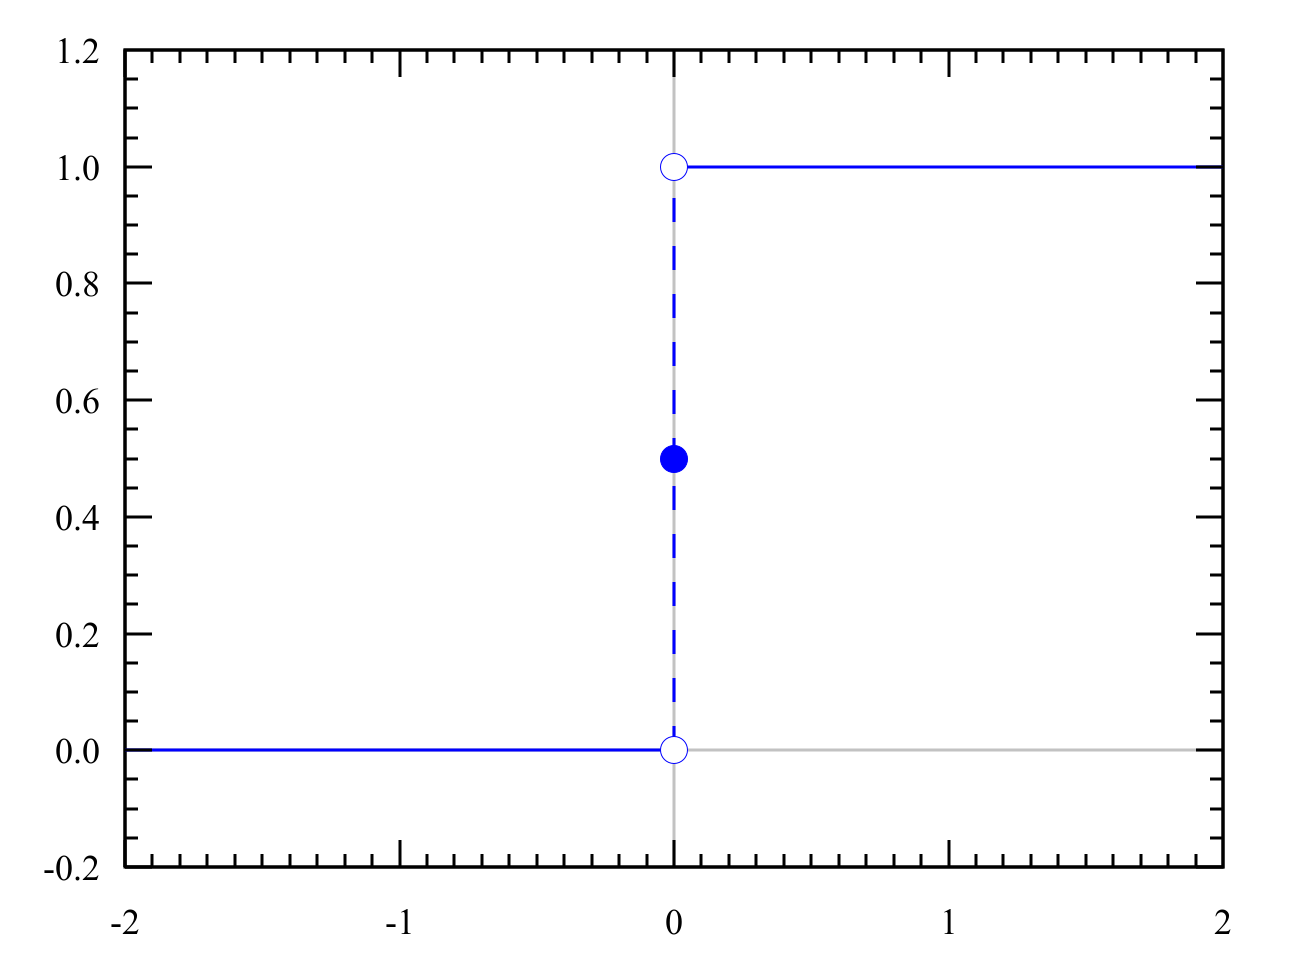
\includegraphics[width=0.85\linewidth]{figure/step.png}
    \caption{Step activation function}
    \label{fig:step}
  \end{minipage}%
  \begin{minipage}{.5\textwidth}
    \centering
    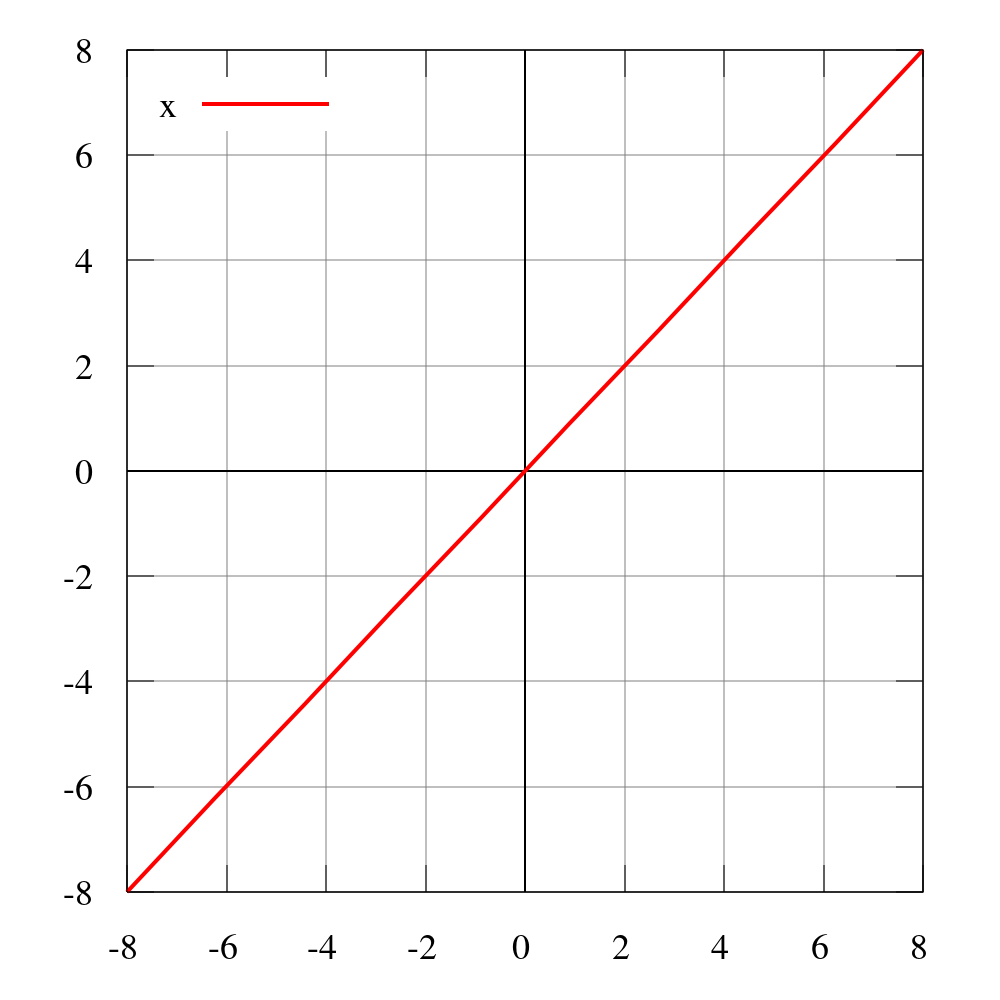
\includegraphics[width=0.75\linewidth]{figure/linear.png}
    \caption{Linear activation function}
    \label{fig:linear}
  \end{minipage}
\end{figure}

\paragraph{Sigmoid}
is a non-linear function defined in the following way:
\begin{center}
  \begin{equation}
    f(x) = \frac{1}{1+e^{x}}
  \end{equation}
\end{center}
The advantages are the smooth gradient that prevents out-of-scale output values, the implicit normalization bound from $[0, +1]$ and the cleaning of the forecast. The main drawback is the vanishing of the gradient, for very high or low input value there is no change in the prediction output, the sigmoid is also computationally expensive. The figure \ref{fig:sigmoid} show the curve.

\paragraph{ReLU} that stand for Rectified Linear Unit and is defined in the following way:
\begin{center}
  \begin{equation}
    f(x)= max(0, x)
  \end{equation}
\end{center}

Although it looks like a linear function, ReLU has a derivative function and allows for backpropagation another advantage is that is computationally efficient. The main problem of this function is its behavior with a value near zero or even negative, the gradient of the function becomes zero and the network can't perform backpropagation and can't learn.

\begin{figure}
  \centering
  \begin{minipage}{.5\textwidth}
    \centering
    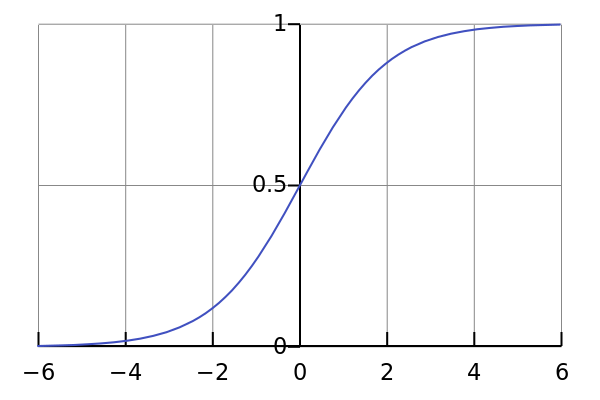
\includegraphics[width=0.8\linewidth]{figure/sigmoid.png}
    \caption{Sigmoid curve}
    \label{fig:sigmoid}
  \end{minipage}%
  \begin{minipage}{.5\textwidth}
    \centering
    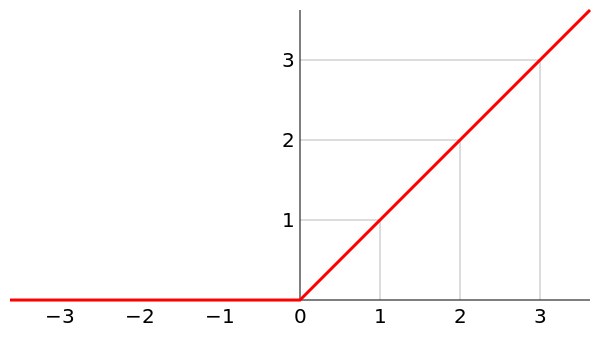
\includegraphics[width=0.8\linewidth]{figure/relu.png}
    \caption{ReLU activation function}
    \label{fig:relu}
  \end{minipage}
\end{figure}

\paragraph{Delta learning rule} uses the difference between target output and the obtained activation to drive the learning. According to these rules, each time an output is computed, the weight of the neuron is adjusted according to an error function trying to reduce the difference between output and target.

\paragraph{Backpropagation} short for \textit{"backward propagation of errors"}, is an algorithm for supervised learning of artificial neural networks using gradient descent. Given an artificial neural network and an error function, the method calculates the gradient of the error function concerning the neural network's weights. It is a generalization of the delta rule for perceptrons to multilayer feedforward neural networks. \cite{bp}.\\
The main characteristic of this technique is that the gradient, proceeds backward through the network, with the gradient of the final layer calculated before the first. This solution allows an efficient calculation of the gradient for each layer. The algorithm is structured in this form:
\begin{enumerate}
  \item Compute the error term for the output units
  \item From the output layer, repeat until last hidden reached:
  \begin{enumerate}
    \item Propagating the error term back to the previous layer
    \item Updating the weights between the two layers
  \end{enumerate}
\end{enumerate}
BP suffers the Vanishing Gradient problem, more layers are embedded in the network and more difficult become to train it. Due to the nature of the backpropagation, when an output is generated, the weight of the neurons is fixed according to the rule, each layer back the correction value is smaller, following the derivate of the activation function, in case of shallow network this problem is solved easily, for deep network this can become a real issue. The ReLU activation function manages better this problem. Another solution is the batch normalization, that rescale the input value between $[-1,1]$ in order to keep the input value far from the activation function edges. Exist a kind of network, Long Short Term Memory, developed to mitigate the vanishing gradient problem, will be discussed later.

\paragraph{Recurrent Neural Networks (RNN)}  is a class of NN that keeps connections between nodes and a temporal sequence. The main difference, respect NN, is that it has feedback connections, this memory allows us to keep track of temporal dynamic behavior, they can process a single data point or the entire sequence of data, like video or speech. They become useful as their intermediate values can store information about past inputs for a time that is not fixed a priori.\\
This kind of structures is used in a lot of different fields: image classification, captioning, sentiment analysis, machine translation, video classification, etc\dots

\paragraph{Long Short Term Memory (LSTM)} normal recurrent neural networks can connect short term event with the present, this feature can be useful in some case, another context could require more long term connection, this special RNN can handle this sort of correlations. Sometimes the recent information is enough to perform the present task, for example, trying to predict the last word of a sentence like "Sun bright in the \textit{sky}" the previous words are enough to correctly predict the last one, no more context is required. In case of more complex sentences some additional information is needed, for the phrase: "I was born in Italy and I speak \textit{italian}" the context becomes fundamental to solve the problem. In this kind of problem LSTM can be really helpful.\\
LSTM are a special kind of RNN, they were introduced by Hochreiter \& Schmidhuber (1997) \cite{lstm} and later studied and improved. It works really well on a large variety of problems. The special kind of network is explicitly designed for long term connections.
The structure of a RNN is normally a single layer, in case of LSTM the structure is more complicated, is made upon four different layers, as shown in figure \ref{fig:lstm}.

\begin{figure}[!ht]
  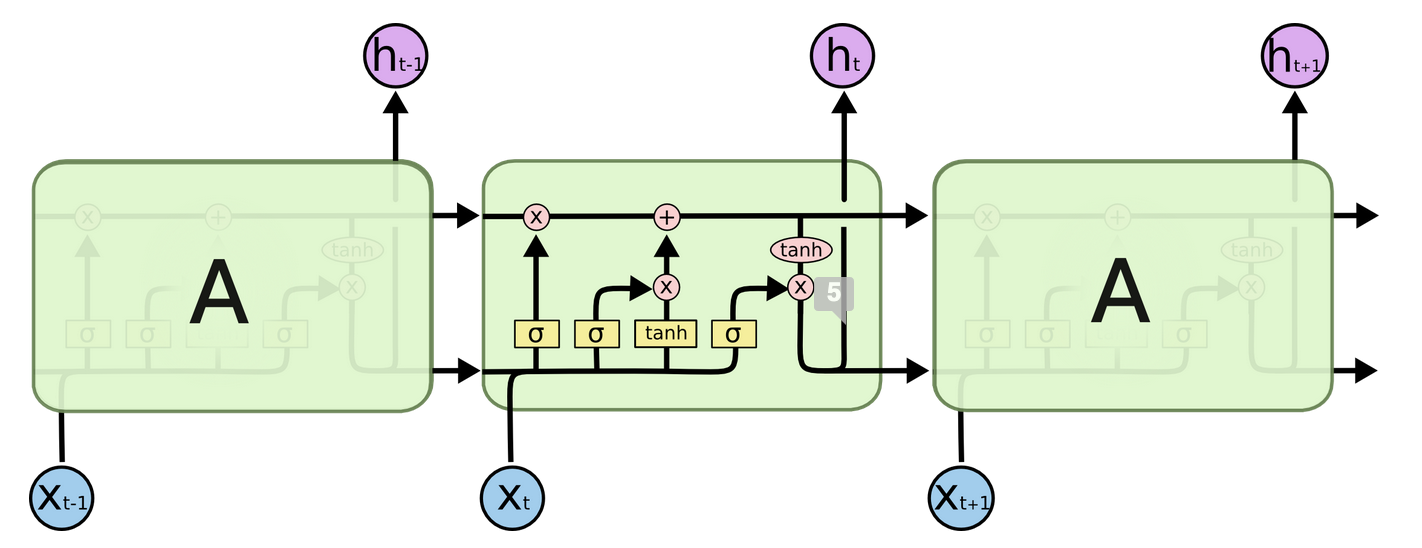
\includegraphics[width=\linewidth]{figure/lstm.png}
  \caption{Long Short Term Memory layout \cite{lstm_image}}
  \label{fig:lstm}
\end{figure}

The first layer filter the input and select what keep and not keep, the second layer will manage what information store in the cell state. The third state is in charge of update the state based on the previous step. The last one decide the output.


\section{Metriche di valutazione}
Every model developed need to be evaluated, there are a lot of different methods that can be used to get metrics about the quality of the system behavior. The computation of these values is achieved via mathematical expression, for this reason, the results, are not always human-readable, some errors like mean absolute error, mean relative error and similar can be read and interpreted without any problem. For metrics like R2 or mean squared error the task becomes more complicated. The following is about the mathematical analysis and description of the different metrics used.\\
Most of metrics directly derive from the calculation of the simplest error, the \textit{absolute error}, the difference between the target $y$ and the prediction $x$:
\begin{center}
  \begin{equation}
    \epsilon = |y - x|
  \end{equation}
\end{center}
Besides being the easiest to calculate is also the easiest to be understand because show directly the distance respect the desired value.\\
The first metric based on the previous metric is the \textit{relative error}, that is computed dividing the absolute error by the target value:
\begin{center}
  \begin{equation}
    \eta = \frac{\epsilon}{|x|} = \frac{|y - x|}{|x|}
  \end{equation}
\end{center}
This error rescale the output between [0,1] in order to better understand the error in the estimation.
For example, in case of a value target value of 530 and a prediciton value of 570 the two error are:
\begin{center}
  \begin{equation}
      \epsilon = |520-570| = 50
  \end{equation}
  \begin{equation}
      \eta = \frac{50}{|520|} = 0.09
  \end{equation}
\end{center}
the difference was 50, but respect the expected output di difference is really low, around 9\%.\\
The previous errors are the basic ones, the following is the first based on aggregation of multiple errors calculation. The aggregation is fundamental to generate a single number to evaluate the quality of prediction of our model.\\
The \textit{Mean Absolute Error} (MAE), is probably the easiest to be calculated and understand, is basically computed by calculating the average of all the absolute errors:

\begin{center}
  \begin{equation}
    MAE = \frac{\sum_{i=1}^{n}{|y_{i} - x_{i}|}}{n} = \frac{\epsilon}{n}
  \end{equation}
\end{center}


% #######################################
% #             Forecasting             #
% #######################################

\chapter{Predizione}
\label{chap:forecasting}
% \section{Introduction}
% Forecasting is the process of making predictions of future based on past and present data by trends analysis. Forecasting is one of the most desired machine learning functionality, it could be used to improve each kind of process, from finacials to production ones. Of course this task is not easy to achieve, a lot of resources and studies are needed to accomplish it.
% The software development is identical to a product development process, starts from the ideation and ends with the production itself.
% The goal is to predict the defectiveness in order to efficently allocate the development effort.

% \section{Features}
% The main advantage, in data analysis, of machines is that they can compute a lot of different data and finding a lot of patterns and correlation that human can't find. Combine the human attitude of logical correlations and machines capacity of number analysis can drive to a powerful combination that can drastically improve the forecasting ability.
% Each artificial intelligence algorithms require a correct and properly studied data in order to perform a valuable prediction, one of the basic step is the data preparation, providing correct and organized data is fundamental to correctly fit the network over the problem.

% \section{Models detail}
% \section{One-Shot Prediction}
% \section{Recurrent forecasting}
% \section{Results}


% % #######################################
% % #         Model abstraction           #
% % #######################################

% \chapter{Model abstraction}
% % \section{CommonDB}
% \section{SFBS and literature comparisons}
% \section{SFFD}


% #######################################
% #             Conclusion              #
% #######################################

\chapter{Conclusioni}
Speaking about conclusion.


% #######################################
% #            BIBLIOGRAPHY             #
% #######################################
\bibliography{biblio}
\bibliographystyle{QUICKtran}


\end{document}
